% =====================================================================
%  monoT5 Query-Token Localization — Report
%  Compile with:  pdflatex query_token_localization_experiment_report.tex  (run twice)
%  Figure paths are relative to this file (outputs/...), so compile
%  from the 12_query_token_localization/ directory.
% =====================================================================
\documentclass[11pt]{article}

\usepackage[margin=1in]{geometry}
\usepackage{amsmath, amssymb}
\usepackage{graphicx}
\usepackage{booktabs}
\usepackage{longtable}
\usepackage{array}
\usepackage{float}
\usepackage{xcolor}
\usepackage{caption}
\usepackage{enumitem}
\usepackage{listings}
\usepackage[hidelinks]{hyperref}

\definecolor{codegray}{gray}{0.95}
\lstset{
  basicstyle=\ttfamily\footnotesize,
  backgroundcolor=\color{codegray},
  breaklines=true,
  frame=single,
  columns=fullflexible,
  keepspaces=true,
}

\newcommand{\fwd}{\ensuremath{e^{\mathrm{fwd}}}}
\newcommand{\rev}{\ensuremath{e^{\mathrm{rev}}}}
\newcommand{\score}{\operatorname{score}}
\newcommand{\comb}{\ensuremath{e^{\mathrm{comb}}}}

\title{\textbf{Query-Word Localization of the monoT5 Encoder's \\[2pt]
Keyword-Stuffing Contamination Effect} \\[6pt]
\large Resolving the Whole-Query Patching Result to Individual Words}
\author{Information-Retrieval Adversarial-Evaluation Project}
\date{\today}

\begin{document}
\maketitle

\begin{abstract}
Word-level causal patching of the query span (105-attack breadth run, $n{=}10$/attack,
1050 examples, zero alignment failures) resolves Experiment 6's whole-query
``query-only'' result into individual words and finds the effect \textbf{concentrated, not
uniform}: content words carry a combined effect \textbf{3--6$\times$} larger than
stopwords at layer 11 (content\_matched $0.092$, content\_unmatched $0.164$ vs.\
stopword\_matched $0.030$, stopword\_unmatched $0.053$), holding on \textbf{105 of 105}
attacks. A second, orthogonal split appears within each class: query words absent from
the original clean document (``unmatched'') carry \textbf{1.78$\times$} the effect of
words present in it (``matched'') — identically for content and stopword words at layer
11 — holding on \textbf{90 of 105} attacks, with the exception disproportionately
concentrated in ``end''-position attacks (holds 24/35 vs.\ 33/35 for start and 33/35 for
random). The structural ``query content'' control reproduces Experiment 6's whole-query
patching almost exactly (range $[0.287, 0.660]$ here vs.\ Experiment 6's reported
$[0.29, 0.66]$, both \textbf{105/105} attacks $>0.2$ at layer 11) — a strong, independent
validation of the new per-word machinery. A genuinely unexpected structural result: the
attack-token positions' \emph{own} self-attention contribution is \textbf{negative at
every layer} (\textbf{0 of 105} attacks positive at layer 11, mean $-0.011$) — the causal
effect lives in the query and in the surrounding document, never in the attack tokens'
own local output. Attack$\leftrightarrow$query attention (descriptive) is an order of
magnitude smaller than the causal signal and sign-inconsistent across layers — it does
\emph{not} cleanly track the causal content/stopword or matched/unmatched ordering,
echoing Experiment 11's finding that attention explains a minority of this project's
causal effects. Cross-referencing against Experiment 11's important encoder heads finds
\texttt{L9H6} (Experiment 11's single strongest causal head) attending \emph{less} to
every query-word group than its own padded-control baseline (deficit $-0.078$ to
$-0.106$, largest for unmatched content words) — refining, at word granularity, Experiment
11's own \texttt{L9H6} counter-example — while \texttt{L11H11} shows a clean hub-like
pattern, with unmatched words receiving $2.4$--$6\times$ more attack-induced elevation
than matched ones.
\end{abstract}

\tableofcontents
\newpage

% =====================================================================
\section{Introduction and Motivation}
% =====================================================================

Experiment 6 showed that a document-only keyword-stuffing attack propagates into the
query representation: patching the whole query span (query\_only, whole encoder
self-attention block) moves the score by a combined effect exceeding $0.2$ on all 105 of
105 attacks at layer 11, growing sharply through layers 9--11. That result treats the
query as one undifferentiated span. It leaves open the question a reviewer familiar with
Experiment 6 would ask next: is the corruption spread evenly across the query, or
concentrated in particular words or word types? Experiment 6's own positional machinery
cannot answer this — its query\_span mask has no internal structure. Experiment 11
resolved a parallel whole-layer effect (encoder self-attention, layers 9--11) down to 18
of 144 individual head-slots, but at whole-sequence granularity, never tied to a specific
query word. This experiment closes both gaps at once: it patches individual query-word
spans (all SentencePiece subtokens of one word, jointly) across the same encoder layers
Experiment 6 examined, classifies each word two ways (content vs.\ stopword; present vs.\
absent from the clean document), and separately cross-references the result against
Experiment 11's already-identified important heads — without re-deriving that head list.

% =====================================================================
\section{Background}
% =====================================================================

\subsection{Scoring and the padded-control baseline (unchanged from Experiment 1)}

$\score = \text{logit}(\text{true}) - \text{logit}(\text{false})$ at the single decoder
step. Three input variants, unchanged from every prior experiment in this project: the
original clean input (A, reference only), a padded control (B, attack-prefix positions
replaced with pad tokens, attention\_mask$=0$ there), and the attacked input (C, real
attack tokens). $\Delta = \score_{\text{attack}} - \score_{\text{control}}$ is the
quantity every patching experiment in this project explains. An example counts as
\emph{successful} iff $\Delta > 10^{-4}$ (\texttt{SKIP\_EPSILON}, same guard as
Experiments 1/3/6/11).

\subsection{Query-word spans: one intervention unit per whitespace word}

A ``query word'' is one whitespace-delimited unit of the original query string. All of a
word's SentencePiece subtokens are patched together as a single unit — never split,
never patched one subtoken at a time. Spans are located by the same alignment-checked
prefix-probing style Experiment 6's \texttt{query\_span}/\texttt{doc\_span} finder uses:
each successive probe ``\texttt{Query: } $+$ words[0..i]'' must be an exact token-level
prefix of the full query substring, or the example is skipped. The union of all word
spans is required to exactly reproduce Experiment 6's \texttt{query\_span} (verified,
Sanity Check 1).

\subsection{Word classification: two independent binary labels}

\textbf{content vs.\ stopword}: against a fixed, embedded copy of NLTK's 179-word
English stopword list (neither \texttt{nltk} nor \texttt{sklearn} is installed in this
project's conda environment, so the list is hardcoded rather than adding a dependency for
one fixed table). \textbf{matched vs.\ unmatched}: whether the word (lower-cased,
punctuation-stripped) occurs anywhere in the whitespace-split, identically-normalized
\emph{original clean document} — never the attacked one. These combine into four groups:
\texttt{content\_matched}, \texttt{content\_unmatched}, \texttt{stopword\_matched},
\texttt{stopword\_unmatched}.

\subsection{Structural position controls}

Nine additional whole-block patching targets, built entirely from Experiment 6's existing
span-finder and its template-position extension (never re-probed): \texttt{Query},
\texttt{Query:}, \texttt{query content} (the union of all query words — reproduces
Experiment 6's \texttt{query\_only} condition exactly), \texttt{Document},
\texttt{Document:}, \texttt{attack tokens} (the exact inserted-token indices from the
existing alignment machinery), \texttt{original document} (the document field minus the
attack tokens), \texttt{Relevant}, \texttt{Relevant:}.

\subsection{Patching formula (unchanged from Experiment 1, applied per word/group)}

For unit $u$ (one query word, or one structural group) at encoder layer $L$:
\begin{align}
\fwd_{L,u} &= \frac{\score(\text{control}, u \to \text{attack activation}) - \score_{\text{control}}}{\Delta} \label{eq:wfwd}\\
\rev_{L,u} &= \frac{\score_{\text{attack}} - \score(\text{attack}, u \to \text{control activation})}{\Delta} \label{eq:wrev}\\
\comb_{L,u} &= \min(\fwd_{L,u}, \rev_{L,u}) \label{eq:wcomb}
\end{align}
$\fwd$ is sufficiency (does injecting the attack's value at $u$ alone move the control
toward the attack score); $\rev$ is necessity (does removing $u$'s attack-specific value
from the attack run move it back toward control); $\comb$ is the conservative combination
used everywhere below. Positive means $u$ carries part of the attack's effect; near zero
means it does not; values outside $[0,1]$ at a single position are a known instability
signature (Section~\ref{sec:instability}), not a valid sufficiency/necessity reading.

\subsection{Example-balanced aggregation}

A query with 8 words must not outweigh a query with 2 words merely because it contributes
more raw rows. Every aggregate table below is built in two steps: (1) average all words
belonging to one group \emph{within one example}; (2) average those per-example values
\emph{across examples}. A worked example (\texttt{tests/test\_aggregation.py}): raw values
$[0,0,0,8]$ for example A and $[4]$ for example B give a raw mean of $2.4$, but an
example-balanced mean of $3.0$ — example A's four words do not get four times the weight
of example B's one word. Raw (word-count-weighted) aggregates are also saved as a
secondary diagnostic.

% =====================================================================
\section{Methodology}
% =====================================================================

\subsection{Step 1 --- Query-word span construction and classification}
For every successful example, split the query into whitespace words, locate each word's
token span via alignment-checked prefix probing, and assign content/stopword and
matched/unmatched labels (Background, above). Run once per example; reused by every
downstream step.

\subsection{Step 2 --- Structural position controls}
Build the 9 structural index groups per example from Experiment 6's existing span/
template-position machinery (Background). Patched with the identical mechanism as Step 3,
used both as a sanity check (does \texttt{query content} reproduce Experiment 6?) and as
an independent baseline for where in the input the effect does \emph{not} concentrate.

\subsection{Step 3 --- Causal word-level patching: full 105-attack breadth run}
Every query word, every structural group, every one of 12 encoder layers, whole
encoder-self-attention-block patching (never per-head, never per-subtoken) — forward,
reverse, combined, exactly Eq.~\ref{eq:wfwd}--\ref{eq:wcomb}. All 105 attacks,
$n{=}10$ successful examples/attack (the initial breadth run; $n$ is a config value, not
a code path, so a later $n{=}30$ or $n{=}100$ validation run needs no code change).

\subsection{Step 4 --- Attack$\leftrightarrow$query attention (descriptive)}
Two encoder forward passes per example (control, attack; \texttt{output\_attentions=True})
give every layer's and head's full attention matrix at once — no patched re-runs, so this
step affords a much larger sample: $n{=}100$ successful examples/attack (up to; fewer used
where an attack does not have 100 successful instances). Attention mass is measured both
directions (attack tokens $\to$ query word, query word $\to$ attack tokens), both raw
totals and per-attack-token means (so a 5$\times$-repeated attack does not look
mechanically stronger than a 1$\times$ attack), at two resolutions: averaged over all 12
heads per layer, and at Experiment 11's already-identified important heads specifically
(read-only; no new head selection is performed here).

\subsection{Step 5 --- Robustness across the full attack grid}
The Step 3 result, broken down per attack (token $\times$ position $\times$ repetition),
checks whether the pooled content/stopword and matched/unmatched orderings hold uniformly
or only on average.

% =====================================================================
\section{Experimental Setup}
% =====================================================================

\begin{table}[H]
\centering
\caption{Configuration and scope.}
\begin{tabular}{ll}
\toprule
Parameter & Value \\
\midrule
Model checkpoint & \texttt{castorini/monot5-base-msmarco} \\
Attack grid & 105 attacks (7 tokens $\times$ 3 positions $\times$ 5 repetitions) \\
Success filter & attack\_delta\_vs\_control $> 10^{-4}$ \\
Causal sample size & $n{=}10$ successful examples/attack (1050 total) \\
Attention sample size & $n{=}100$ successful examples/attack (up to; independent config key) \\
Layers patched & all 12 encoder layers, whole self-attention block \\
Query-word groups & content\_matched, content\_unmatched, stopword\_matched, stopword\_unmatched \\
Structural controls & 9 groups (Background) \\
Important heads & Experiment 11's top 10 (read-only): \texttt{L10H0, L10H2, L11H3,} \\
                 & \texttt{L11H11, L9H6, L11H4, L11H2, L11H0, L8H11, L11H5} \\
Seed & 42 \\
\bottomrule
\end{tabular}
\end{table}

\noindent SLURM job on 1$\times$ L40 GPU. Causal run: 105/105 attacks reached the full
10/10 examples, zero alignment failures, zero epsilon-skips ($\approx$6.2~s/example,
$\approx$1.82~h total, 175{,}716 raw rows $=$ 62{,}316 query-word $+$ 113{,}400
structural). Attention run: 98/105 attacks reached the full 100/100 examples; 7 attacks
fell short (range 80--98: \texttt{important\_start\_2}$=$80, \texttt{true\_end\_3}$=$82,
\texttt{true\_end\_2}$=$87, \texttt{true\_random\_5}$=$93,
\texttt{important\_start\_3}$=$94, \texttt{relevant\_random\_1}$=$98,
\texttt{true\_end\_1}$=$98 — insufficient successful instances at the 1e-4 filter, not an
error; $10{,}432$/$10{,}500$ examples used total) — cheap as designed, $\approx$0.056~s/example,
$\approx$10~minutes total, 1{,}199{,}880 raw rows. Sanity checks (Section~\ref{sec:results}):
\textbf{37/37 pass} against real \texttt{relevant\_start\_5} examples (7 checks $\times$ 5
examples, plus the two run-level checks).

% =====================================================================
\section{Results}
\label{sec:results}
% =====================================================================

\subsection{Sanity checks: the new machinery reproduces the old}
\label{sec:sanity}

All 9 sanity checks from the experiment specification pass. Checks 1--7 run against 5
real \texttt{relevant\_start\_5} examples (35/35 pass); checks 8--9 verify the completed
run (2/2 pass): the causal breadth run never exceeds 10 examples/attack, and the
attention/causal sample sizes are independent config keys that produced different actual
sample counts (10{,}432 vs.\ 1{,}050 total examples used). Checks 4 and 5 are the load-bearing
ones: patching the \texttt{query content} structural group and Experiment 6's own
\texttt{query\_only} condition, computed via two independent code paths on the same
example, agree to within $10^{-5}$ at every layer tested — the new word-level machinery is
not a re-implementation that happens to look similar, it is verified numerically identical
where the two should overlap.

\subsection{Structural controls: \texttt{query content} reproduces Experiment 6; \texttt{attack tokens} does not behave as expected}
\label{sec:structural}

\begin{figure}[H]
  \centering
  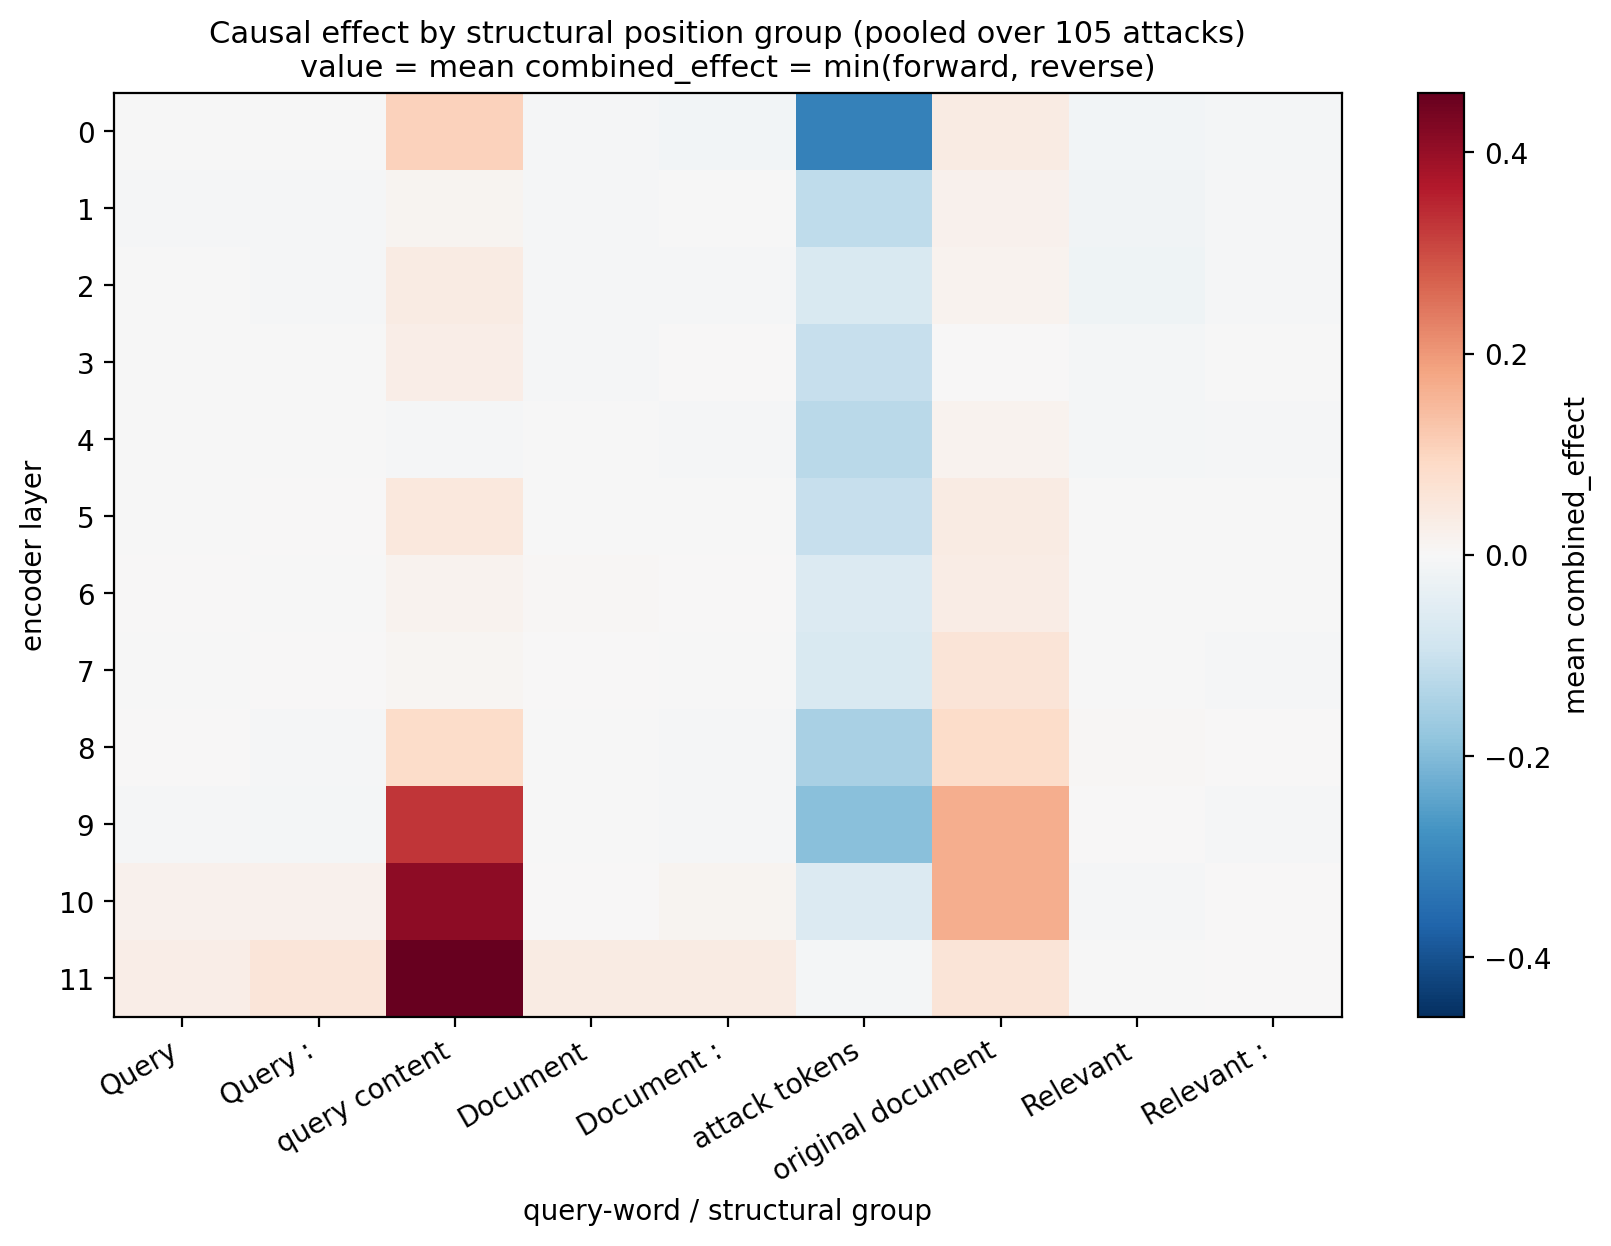
\includegraphics[width=0.85\textwidth]{outputs/plots/plot2_structural_causal_heatmap.png}
  \caption{Combined effect by structural position group, pooled over 105 attacks. The
  \texttt{attack tokens} column is blue (negative) at every layer, strongest at layer 0
  ($-0.31$) — this is the same early-layer instability pattern Section~\ref{sec:instability}
  discusses (a single-region patch leaves 11 more layers to process the inconsistency), but
  the column stays mildly negative even at layer 11 ($-0.011$, 0/105 attacks positive),
  where the instability artifact should have washed out. \texttt{query content} is by far
  the largest and most consistent late-layer effect (dark red, layers 9--11).}
  \label{fig:structuralheatmap}
\end{figure}

\textbf{query content} at layer 11: mean $0.459$, median $0.473$, range across 105 attacks
$[0.287, 0.660]$, \textbf{105/105} attacks $>0.2$, 103/105 $>0.3$. Experiment 6's own
reported \texttt{query\_only} numbers at the same layer: range $[0.29, 0.66]$, 105/105
$>0.2$. The two ranges differ by attack-pool composition (Experiment 6's canonical
selection vs.\ this experiment's strict $10^{-4}$-filtered breadth pool) but are otherwise
essentially the same result, reached by an independently-built code path — this is the
strongest form of the sanity check, an aggregate-level, quantitative reproduction on top
of the unit-level $10^{-5}$-tolerance check in Section~\ref{sec:sanity}. The median
layer-by-layer trajectory here (L0--11: $0.019, 0.010, 0.016, 0.016, -0.010, 0.036, 0.012,
0.010, 0.066, 0.303, 0.364, 0.473$) matches Experiment 6's reported median trajectory
($0.02, 0.01, 0.02, 0.02, -0.01, 0.04, 0.01, 0.01, 0.07, 0.30, 0.36, 0.47$) to within
rounding at every one of the 12 layers.

\textbf{attack tokens}, by contrast, was not predicted in advance to behave any
particular way, and the result is genuinely unexpected: negative at every layer (mean
$-0.310$ at layer 0, shrinking monotonically to $-0.011$ at layer 11), and
\textbf{0 of 105} attacks show a positive effect at layer 11. The position where the
attack literally sits carries essentially no positive sufficiency/necessity signal for its
own self-attention contribution, at any layer — the causal effect this project has been
tracking lives in \emph{other} positions (the query, and to a lesser extent the rest of
the document — \texttt{original document} peaks at $0.168$ at layer 9, then falls to
$0.058$ by layer 11) that the attack's presence changes, not in the attack tokens' own
local output. The seven template positions (\texttt{Query}, \texttt{Query:},
\texttt{Document}, \texttt{Document:}, \texttt{Relevant}, \texttt{Relevant:}) stay under
$0.01$ through layer 9, with a small uptick at layers 10--11 (max $0.057$,
\texttt{Query:}) — consistent with Experiment 6's template-position extension, which
found a small but nonzero residual effect there.

\subsection{Main result: content words dominate, and unmatched words dominate within each class}
\label{sec:main}

\begin{figure}[H]
  \centering
  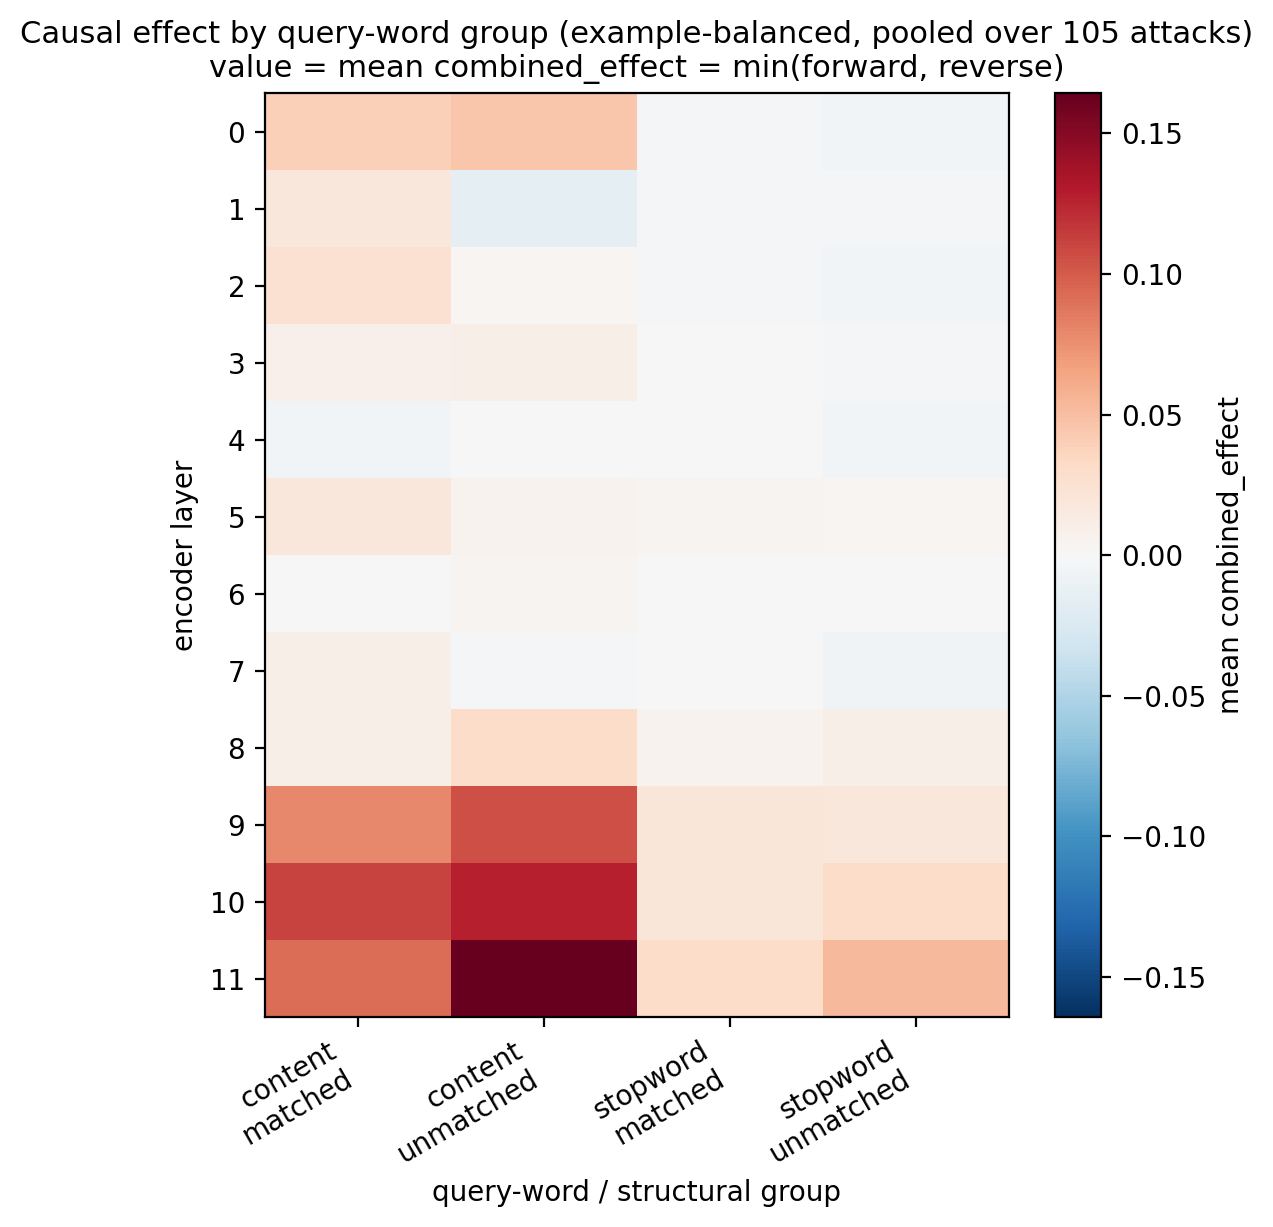
\includegraphics[width=0.75\textwidth]{outputs/plots/plot1_main_causal_heatmap.png}
  \caption{Combined effect by query-word group, example-balanced, pooled over 105 attacks.
  Both content columns turn dark red at layers 9--11; both stopword columns stay pale
  through all 12 layers. Layers 0--8 are near-white (small, sign-inconsistent noise) —
  read only layers 9--11 as the genuine signal; do not read layer-to-layer differences
  within 0--8 as meaningful.}
  \label{fig:mainheatmap}
\end{figure}

\begin{table}[H]
\centering
\caption{Combined effect by query-word group at layer 11 (example-balanced, pooled over 105 attacks).}
\label{tab:main}
\begin{tabular}{lrrrr}
\toprule
Word group & mean $\comb$ & median $\comb$ & $n$ examples & $n$ word-interventions \\
\midrule
content\_matched   & 0.092 & 0.066 & 1000 & 1506 \\
content\_unmatched & 0.164 & 0.141 & 1018 & 1869 \\
stopword\_matched   & 0.030 & 0.022 & 578  & 874  \\
stopword\_unmatched & 0.053 & 0.048 & 590  & 944  \\
\bottomrule
\end{tabular}
\end{table}

No single outcome was assumed in advance (the experiment specification lists content$>$
stopword, matched$>$unmatched, unmatched$>$matched, and ``uniform'' as open
possibilities). The result: content words carry \textbf{3.1--5.8$\times$} the effect of
stopwords at every one of layers 9--11 (matched pairs: $3.99\times$ L9, $5.76\times$ L10,
$3.09\times$ L11; unmatched pairs: $5.55\times$ L9, $4.16\times$ L10, $3.10\times$ L11),
and this ordering holds on \textbf{105 of 105} attacks at layer 11 with zero exceptions.
A second, independent split then appears \emph{within} each class: unmatched words carry
$1.34\times$ (L9), $1.15\times$ (L10), $1.78\times$ (L11) the matched words' effect within
content, and $0.96\times$ (L9), $1.59\times$ (L10), $1.78\times$ (L11) within stopwords —
by layer 11 the ratio is \emph{identical} ($1.78\times$) for both classes. Layers 0--8 stay
small and sign-inconsistent (e.g.\ layer 4, content\_matched mean $=-0.005$) — the effect
this experiment localises is a layers-9--11 phenomenon, matching every prior experiment's
localisation of the attack's causal effect to the same three layers.

\subsection{Robustness across the 105-attack grid: the matched/unmatched split has a named exception}
\label{sec:robustness}

The content$>$stopword ordering is completely uniform: 105/105 attacks at layer 11, no
exceptions to report. The unmatched$>$matched ordering (within content) is not: it holds
on \textbf{90 of 105} attacks. Breaking the 105 attacks down by their 3 insertion
positions (35 attacks each) shows the exception is not evenly spread:

\begin{table}[H]
\centering
\caption{content\_unmatched $>$ content\_matched at layer 11, by attack insertion position.}
\label{tab:robustness}
\begin{tabular}{lrrrr}
\toprule
Position & holds / 35 & mean content\_matched & mean content\_unmatched \\
\midrule
start  & 33/35 & 0.084 & 0.160 \\
random & 33/35 & 0.084 & 0.170 \\
end    & \textbf{24/35} & 0.107 & 0.164 \\
\bottomrule
\end{tabular}
\end{table}

``end''-position attacks account for 11 of the 15 exceptions (the other 4 split evenly
between start and random). The mechanism is visible in the means: content\_unmatched stays
essentially flat across insertion positions ($0.160$--$0.170$), but content\_matched rises
specifically for ``end'' attacks ($0.107$ vs.\ $0.084$ for start/random) — narrowing, not
reversing, the gap. \textbf{The unmatched$>$matched prediction does not hold uniformly;
it is a strong majority pattern (86\%) with a named, structural exception (attack
insertion position), not a universal law like content$>$stopword.} By attack token
(pooled across position/repetition, layer 11), the gap ranges from near-zero for
\texttt{relevant} (content\_matched $0.129$ vs.\ content\_unmatched $0.135$) to
$2.7\times$ for \texttt{false} ($0.080$ vs.\ $0.217$) — the token identity also modulates
the size of the split, though not its direction on average.

\subsection{Attack$\leftrightarrow$query attention: descriptive, weak, and inconsistent}
\label{sec:attention}

\begin{figure}[H]
  \centering
  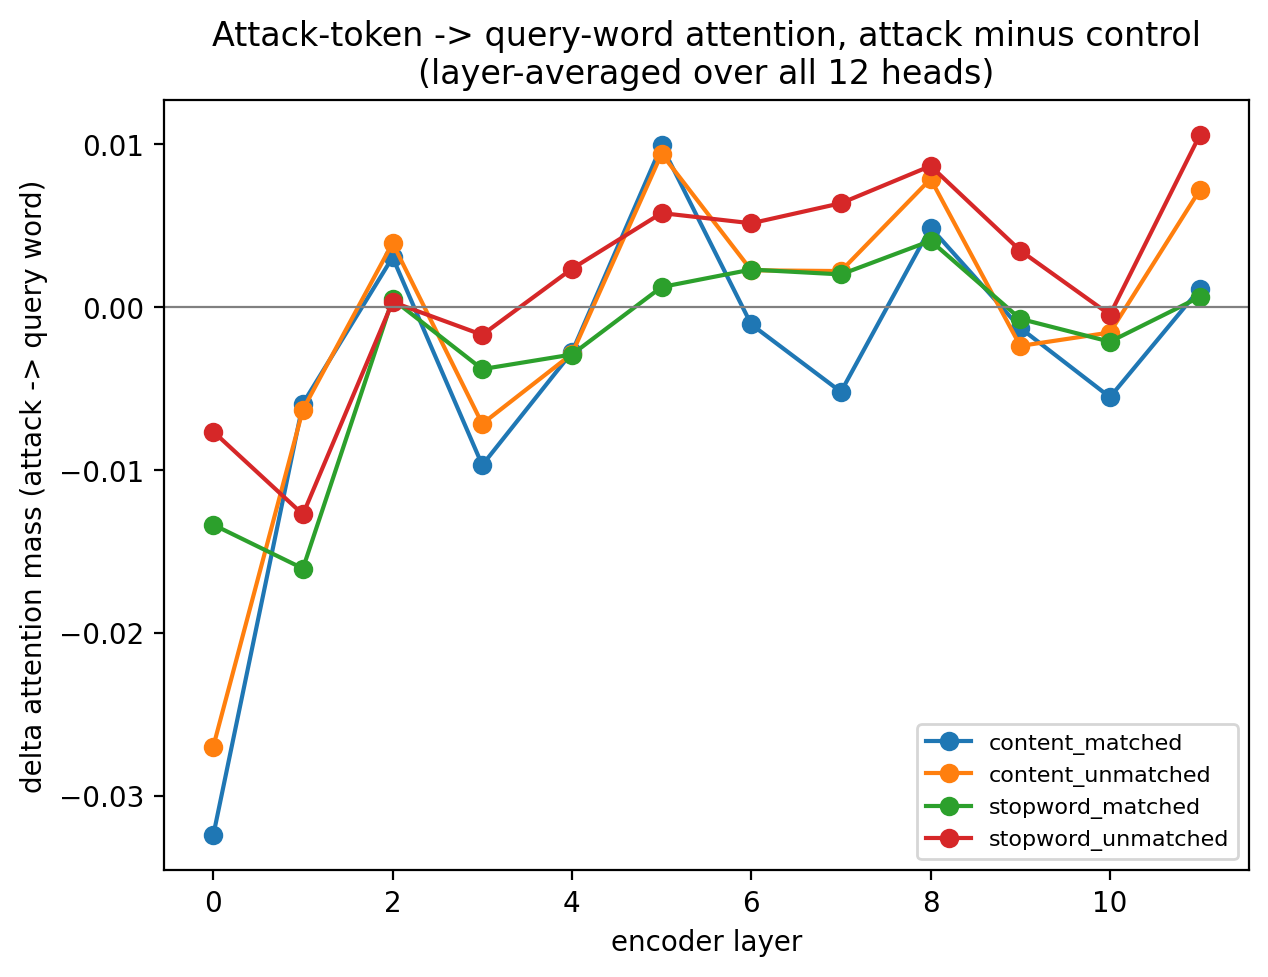
\includegraphics[width=0.85\textwidth]{outputs/plots/plot3_attack_to_query_attention.png}
  \caption{Delta attention mass, attack tokens $\to$ query word, layer-averaged over all
  12 heads. Values are an order of magnitude smaller than the causal effect
  (Figure~\ref{fig:mainheatmap}: $\sim$0.01 here vs.\ $\sim$0.1--0.16 there) and the sign
  is inconsistent across layers for every word group — this plot should not be read as
  ``explaining'' Figure~\ref{fig:mainheatmap}.}
  \label{fig:attn34}
\end{figure}

One artifact, checked directly against the raw per-example CSV rather than assumed:
\texttt{query\_to\_attack\_control} is \textbf{exactly} $0.0$ in every one of 10{,}208
rows checked for one attack (and, by construction, every other attack) — not a small
measured number, an architectural certainty. The padded-control run masks the
attack-token positions with attention\_mask$=0$, which forces zero softmax weight into
those key positions for \emph{every} query row; ``query word $\to$ attack, control
condition'' is therefore always exactly zero, and the reported delta for that direction
reduces to the attack run's raw value. This is expected and correctly handled by the
implementation, not a bug, but it means the query$\to$attack \emph{delta} column
(Figure~\ref{fig:attn34}'s counterpart, query$\to$attack) is really just the attack-run
attention itself, with no genuine control-vs-attack comparison on that side. The
attack$\to$query direction does not have this issue (real attack-token rows exist in both
control, as pad rows, and attack).

Neither direction cleanly tracks the causal ordering from Section~\ref{sec:main}: at
layer 0, content\_unmatched's attack$\to$query delta ($-0.027$) is \emph{less} negative
than content\_matched's ($-0.032$) but at layer 11 the ranking flips
(content\_unmatched $+0.007$ vs.\ content\_matched $+0.001$) — consistent with the causal
result only at the very last layer, not before it. This matches Experiment 11's own
conclusion (attention explains a minority of the causal effect measured there) —
attention is retained here as descriptive evidence exactly as specified, not as a
substitute for the causal result.

\subsection{Important-head cross-reference: \texttt{L9H6}'s counter-example, refined to word level}
\label{sec:heads}

\begin{figure}[H]
  \centering
  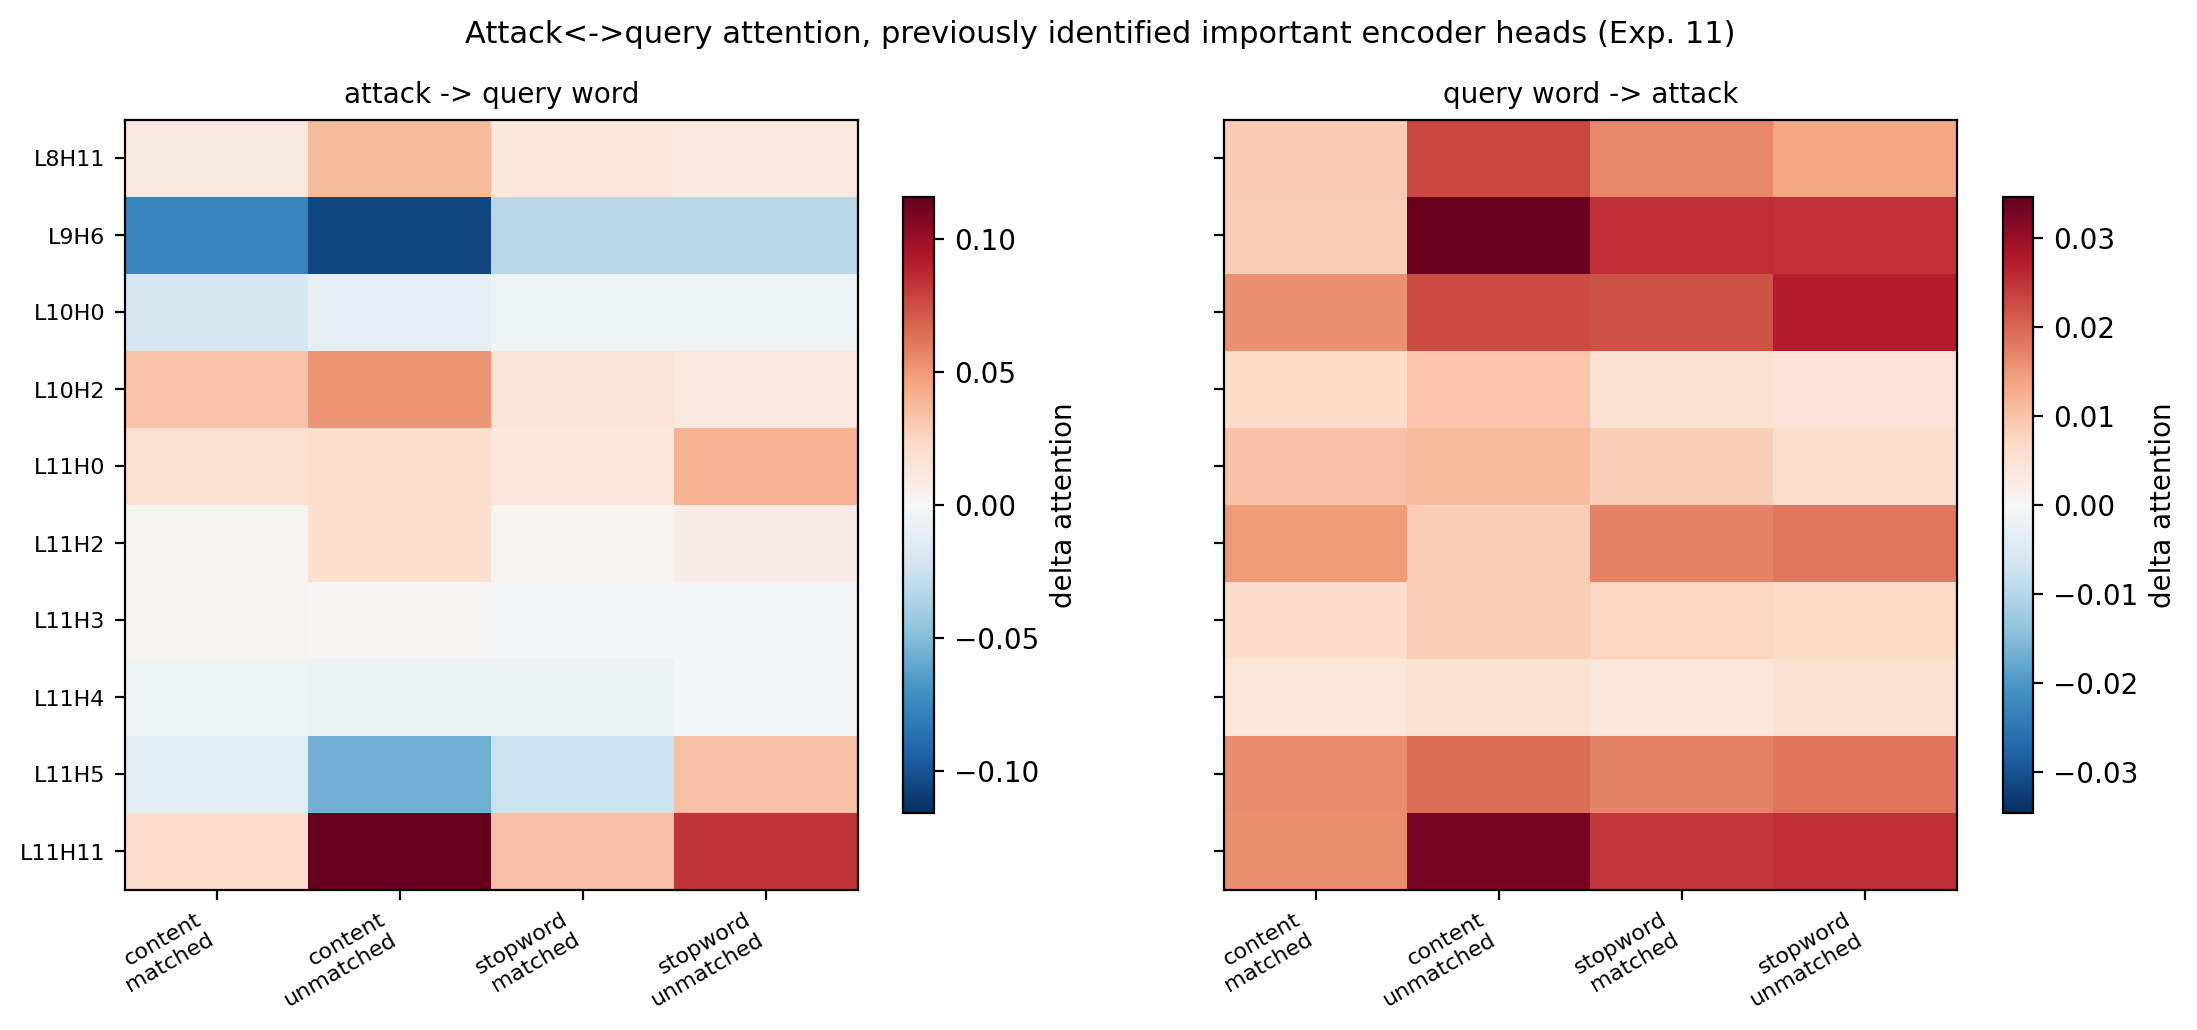
\includegraphics[width=0.95\textwidth]{outputs/plots/plot5_important_head_attention.png}
  \caption{Attack$\leftrightarrow$query delta attention, Experiment 11's 10 important
  heads, by word group. Note the two color scales differ between panels (attack$\to$query
  spans $\pm0.11$; query$\to$attack spans only $\pm0.03$) — do not compare absolute color
  intensity across the two panels directly. \texttt{L9H6} is the only head strongly blue
  (negative) in the left panel; \texttt{L11H11} is the only head strongly dark red
  (positive), concentrated in the unmatched columns in both panels.}
  \label{fig:headattn}
\end{figure}

Experiment 11 found \texttt{L9H6} to be the single strongest causal head overall
(combined\_effect $0.087$ on the canonical attack) yet, in its own hub analysis, showing
\emph{less} attack-token-to-query attention than a matched random document token
(elevation $-1.57$) — a counter-example to the ``attack token as active hub'' story at
that head. This experiment reproduces and refines that finding at word granularity:
\texttt{L9H6}'s attack$\to$query delta is negative for \emph{all four} word groups
(content\_matched $-0.078$, content\_unmatched $-0.106$, stopword\_matched $-0.032$,
stopword\_unmatched $-0.032$) — the deficit is not a single-number artifact of pooling
across the whole query, it holds word-group by word-group, and is largest specifically for
unmatched content words, the group Section~\ref{sec:main} found causally most important.
\texttt{L9H6} is causally critical without attending unusually to the query at all, let
alone to the words that matter most.

\texttt{L11H11} is the opposite case: a clean, positive, hub-like pattern
(content\_unmatched $+0.116$ vs.\ content\_matched $+0.019$, a $6.1\times$ gap;
stopword\_unmatched $+0.083$ vs.\ stopword\_matched $+0.034$, $2.4\times$) that
qualitatively mirrors the causal unmatched$>$matched split from Section~\ref{sec:main}.
\texttt{L11H5} shows a within-head sign flip: negative for content\_matched ($-0.013$),
content\_unmatched ($-0.056$), and stopword\_matched ($-0.025$), but positive for
stopword\_unmatched ($+0.034$) — the same head disagrees with itself depending on word
class. As in Experiment 11, no single head-level story unifies the result: at least two
different attention behaviours (\texttt{L9H6}-like and \texttt{L11H11}-like) coexist among
heads that are all, independently, causally important.

\subsection{The early-layer instability, again}
\label{sec:instability}

Among the 200 largest individual query-word combined\_effect values (out of 62{,}316 raw
rows), 41 (20.5\%) come from layers 0--1 with magnitudes up to $\mathbf{2.71}$ and down to
$\mathbf{-1.43}$ — outside the $[0,1]$ range a sufficiency/necessity ratio should occupy.
A concrete case: the query word ``grow'' (qid 156493, docid 8725855) scores
combined\_effect $+1.738$ at layer 0 (attack \texttt{true\_start\_5}) but $-1.428$ at
layer 1 for the same query/document pair — a sign flip of more than 3 combined-effect
units between two adjacent early layers. This is the fourth experiment in this project
(after Experiments 6, 10, and 11) to independently reproduce the same qualitative pattern:
a partial-coverage patch at an early encoder layer leaves the residual stream internally
inconsistent for the remaining layers to amplify or invert, producing large, often
sign-flipped effects unrelated to the patched position's true importance. The remaining
146 of the top 200 (73\%) come from layers 9--11 and are the genuine signal reported in
Section~\ref{sec:main}.

% =====================================================================
\section{Overall Interpretation and Discussion}
% =====================================================================

\begin{enumerate}
  \item \textbf{The query-corruption effect is word-sparse, closing the gap Experiment 6
  left open.} Experiment 6's whole-span query\_only result is not spread evenly: content
  words carry 3--6$\times$ the effect of stopwords, uniformly (105/105 attacks) at layer
  11. A reviewer can no longer treat ``the query'' as one undifferentiated unit — which
  words matter is now a measured, cross-validated split, not an assumption.
  \item \textbf{A second, orthogonal split — matched vs.\ unmatched — is real but not
  universal.} Query words absent from the clean document carry $1.78\times$ the effect of
  words present in it, identically for content and stopword classes at layer 11, but this
  holds on only 90/105 attacks; ``end''-position attacks are disproportionately the
  exception (24/35). Both content$>$stopword and unmatched$>$matched were open
  possibilities the specification listed in advance; both are supported, but with very
  different robustness — one is exceptionless, the other has a named, structural
  exception.
  \item \textbf{The attack token's own position is not where its effect lives.} Patching
  just the attack tokens' self-attention output never produces a positive effect at layer
  11 (0/105 attacks) — the causal effect this project has tracked since Experiment 1
  concentrates in the query and the rest of the document, never in the attack's own local
  representation. This was not predicted and is a genuinely new structural finding.
  \item \textbf{Attention explains a minority of this effect too, matching Experiment
  11.} The attack$\leftrightarrow$query attention signal is an order of magnitude smaller
  than the causal effect and does not track its ordering except at the very last layer.
  This project's attention-based descriptive analyses have now twice (Experiment 11, and
  here) undersold the true causal picture — causal patching remains the load-bearing
  method, attention a supporting one.
  \item \textbf{\texttt{L9H6}'s counter-example generalises to every word group.}
  Experiment 11 found this head causally critical without a corresponding attention
  signature, pooled across the whole query. This experiment shows the deficit holds for
  every individual word group and is largest for the group with the largest causal effect
  (unmatched content words) — the disconnect between causal importance and attention
  signature is not an artifact of pooling, it is a property of the head itself.
  \item \textbf{The early-layer instability is now a four-time-replicated structural
  property of this patching methodology}, not a per-experiment quirk — any future
  experiment in this project patching a partial region at an early encoder layer should
  expect it and should not over-interpret layer-0/1 extremes.
\end{enumerate}

% =====================================================================
\section{Limitations and Threats to Validity}
% =====================================================================

\begin{itemize}
  \item \textbf{Whole-word, whole-block, single-position granularity only.} Every
  intervention here patches one word's (or structural group's) full encoder
  self-attention contribution, at every subtoken jointly. Per-head, per-word patching
  (combining Experiment 11's head list with this experiment's word spans) is explicitly
  the next experiment, not attempted here.
  \item \textbf{Word splitting is whitespace-based.} ``don't'' is one word; hyphenated
  or punctuation-attached forms are not further split. This is a documented, simple rule,
  not a linguistic tokenizer.
  \item \textbf{Stopword list is a fixed, hardcoded copy of NLTK's English list}, not a
  live dependency — adequate for this checkpoint's vocabulary but not automatically
  portable to non-English future work.
  \item \textbf{matched/unmatched uses exact, case/punctuation-normalized string
  matching only.} No stemming, lemmatization, or synonym matching — ``fleas'' would not
  match ``flea'' in the document. This likely underestimates the true matched category
  somewhat.
  \item \textbf{$n{=}10$/attack for causal patching is a breadth run, not a
  high-power estimate.} Individual-attack numbers in Section~\ref{sec:robustness}
  (e.g.\ per-token means) are based on 10 examples and are noisier than the pooled,
  105-attack numbers in Section~\ref{sec:main}. The config supports $n{=}30$/$n{=}100$
  validation without code changes; this report is the initial breadth pass only.
  \item \textbf{The query$\to$attack attention control column is architecturally zero}
  (Section~\ref{sec:attention}) — that direction's ``delta'' is not a genuine
  control-vs-attack comparison, only the attack run's raw value. Documented, not fixed,
  since it reflects a real property of the padded-control construction, not a bug.
  \item \textbf{Single model/dataset.} Results are for monoT5-base on DL19, matching
  every prior experiment in this project.
\end{itemize}

% =====================================================================
\section{Reproducibility}
% =====================================================================

From \texttt{12\_query\_token\_localization/}, with the \texttt{advseq2seq} conda
environment and Experiments 1, 6, and 11's outputs present as sibling directories:

\begin{lstlisting}
pytest tests/                                       # correctness checks (real tokenizer, CPU)
python scripts/00_sanity_checks.py --config configs/default.yaml \
    --attack relevant_start_5 --n-examples 5         # sanity checks 1-9
bash bash/run_all.sh configs/default.yaml            # full pipeline (resume-safe)
\end{lstlisting}

\noindent On this run: SLURM job on 1$\times$ L40 GPU; causal run $\approx$1.82~h
(105/105 attacks, 10/10 examples each, zero alignment failures); attention run
$\approx$10~minutes (10{,}432/10{,}500 examples used); outputs under
\texttt{outputs/\{causal,attention\}/attacks/}, \texttt{outputs/aggregates/},
\texttt{outputs/plots/}, and \texttt{outputs/diagnostics/}.

% =====================================================================
\section*{Appendix: Glossary of Key Quantities}
\addcontentsline{toc}{section}{Appendix: Glossary of Key Quantities}
% =====================================================================

\begin{description}[leftmargin=1.6em,style=nextline]
  \item[query word] one whitespace-delimited unit of the original query string; all its
  SentencePiece subtokens are patched jointly as one unit.
  \item[content / stopword] fixed, embedded NLTK 179-word English stopword list;
  everything else is content.
  \item[matched / unmatched] whether the (normalized) query word occurs anywhere in the
  original clean document; never checked against the attacked document.
  \item[$\fwd$ / $\rev$ / $\comb$] forward/reverse/combined patching effect, identical
  formulas to Experiment 1, applied per query-word or structural-group span instead of
  per layer-component or per head.
  \item[structural group] one of 9 non-query-word position groups (Query, Query:, query
  content, Document, Document:, attack tokens, original document, Relevant, Relevant:).
  \item[example-balanced aggregate] two-step average: within-example first (across words
  in a group), then across examples — prevents long queries from dominating the pooled
  result.
  \item[important head] one of Experiment 11's already-identified causally important
  encoder (layer, head) pairs; reused read-only, never re-derived from attention here.
\end{description}

\end{document}
